\subsection{Reverse Data}
\subsubsection{Time}
\textbf{Comments on the running time of sorting algorithms with reverse data}
\begin{enumerate}
    \item \textbf{Fastest Algorithms:} \\
- \textit{Heap Sort}, \textit{Radix Sort}, and \textit{Counting Sort} again perform the fastest across all input sizes. Their execution times remain very low even for larger input sizes, similar to their performance on sorted input.

    \item \textbf{Slowest Algorithms:} \\
- \textit{Bubble Sort}, \textit{Shaker Sort}, and \textit{Quick Sort} exhibit very high execution times, especially as the input size increases. For instance, bubble sort's time grows from 76.9914 seconds at 10000 elements to 195572 seconds at 500000 elements.

    \item \textbf{Consistent Performers:} \\
- \textit{Merge Sort} and \textit{Shell Sort} show relatively stable and moderate execution times, indicating reliable performance across different input sizes.
\end{enumerate}

Execution time unit: milliseconds

\begin{table}[h!]
\centering
\begin{tabular}{|l|r|r|r|r|r|r|}
\hline
\textbf{Algorithm} & \textbf{10000} & \textbf{30000} & \textbf{50000} & \textbf{100000} & \textbf{300000} & \textbf{500000} \\
\hline
Selection Sort & 85.285 & 764.617 & 2085.39 & 8471.83 & 75944.1 & 210673 \\ \hline
Insertion Sort & 11.1563 & 100.834 & 276.323 & 1090.38 & 9847.49 & 28014.6 \\ \hline
Shell Sort & 21.0003 & 203.454 & 527.093 & 2115.4 & 18846.1 & 55537.9 \\ \hline
Bubble Sort & 76.9914 & 692.504 & 1928.01 & 7667.36 & 69228.6 & 195572 \\ \hline
Heap Sort & 0.6743 & 2.2238 & 4.1879 & 8.3122 & 26.5599 & 45.5919 \\ \hline
Merge Sort & 2.5089 & 7.4184 & 12.1534 & 23.8237 & 73.346 & 123.387 \\ \hline
Quick Sort & 44.9166 & 400.345 & 1098.21 & 4412.2 & 39600.2 & 112705 \\ \hline
Radix Sort & 0.133 & 0.4967 & 0.8283 & 1.5792 & 5.9777 & 10.3353 \\ \hline
Counting Sort & 0.016 & 0.0421 & 0.0752 & 0.1617 & 0.6948 & 1.2085 \\ \hline
Binary Insertion Sort & 7.9368 & 78.3401 & 204.501 & 795.454 & 7076.07 & 21493.8 \\ \hline
Shaker Sort & 81.9425 & 730.12 & 2068.47 & 8181.6 & 73751.9 & 204937 \\ \hline
Flash Sort & 0.1018 & 0.317 & 0.6843 & 1.3254 & 3.8055 & 6.2582 \\
\hline
\end{tabular}
\label{table:reverse_execution_time}
\end{table}

\begin{figure}[h]
    \centering
    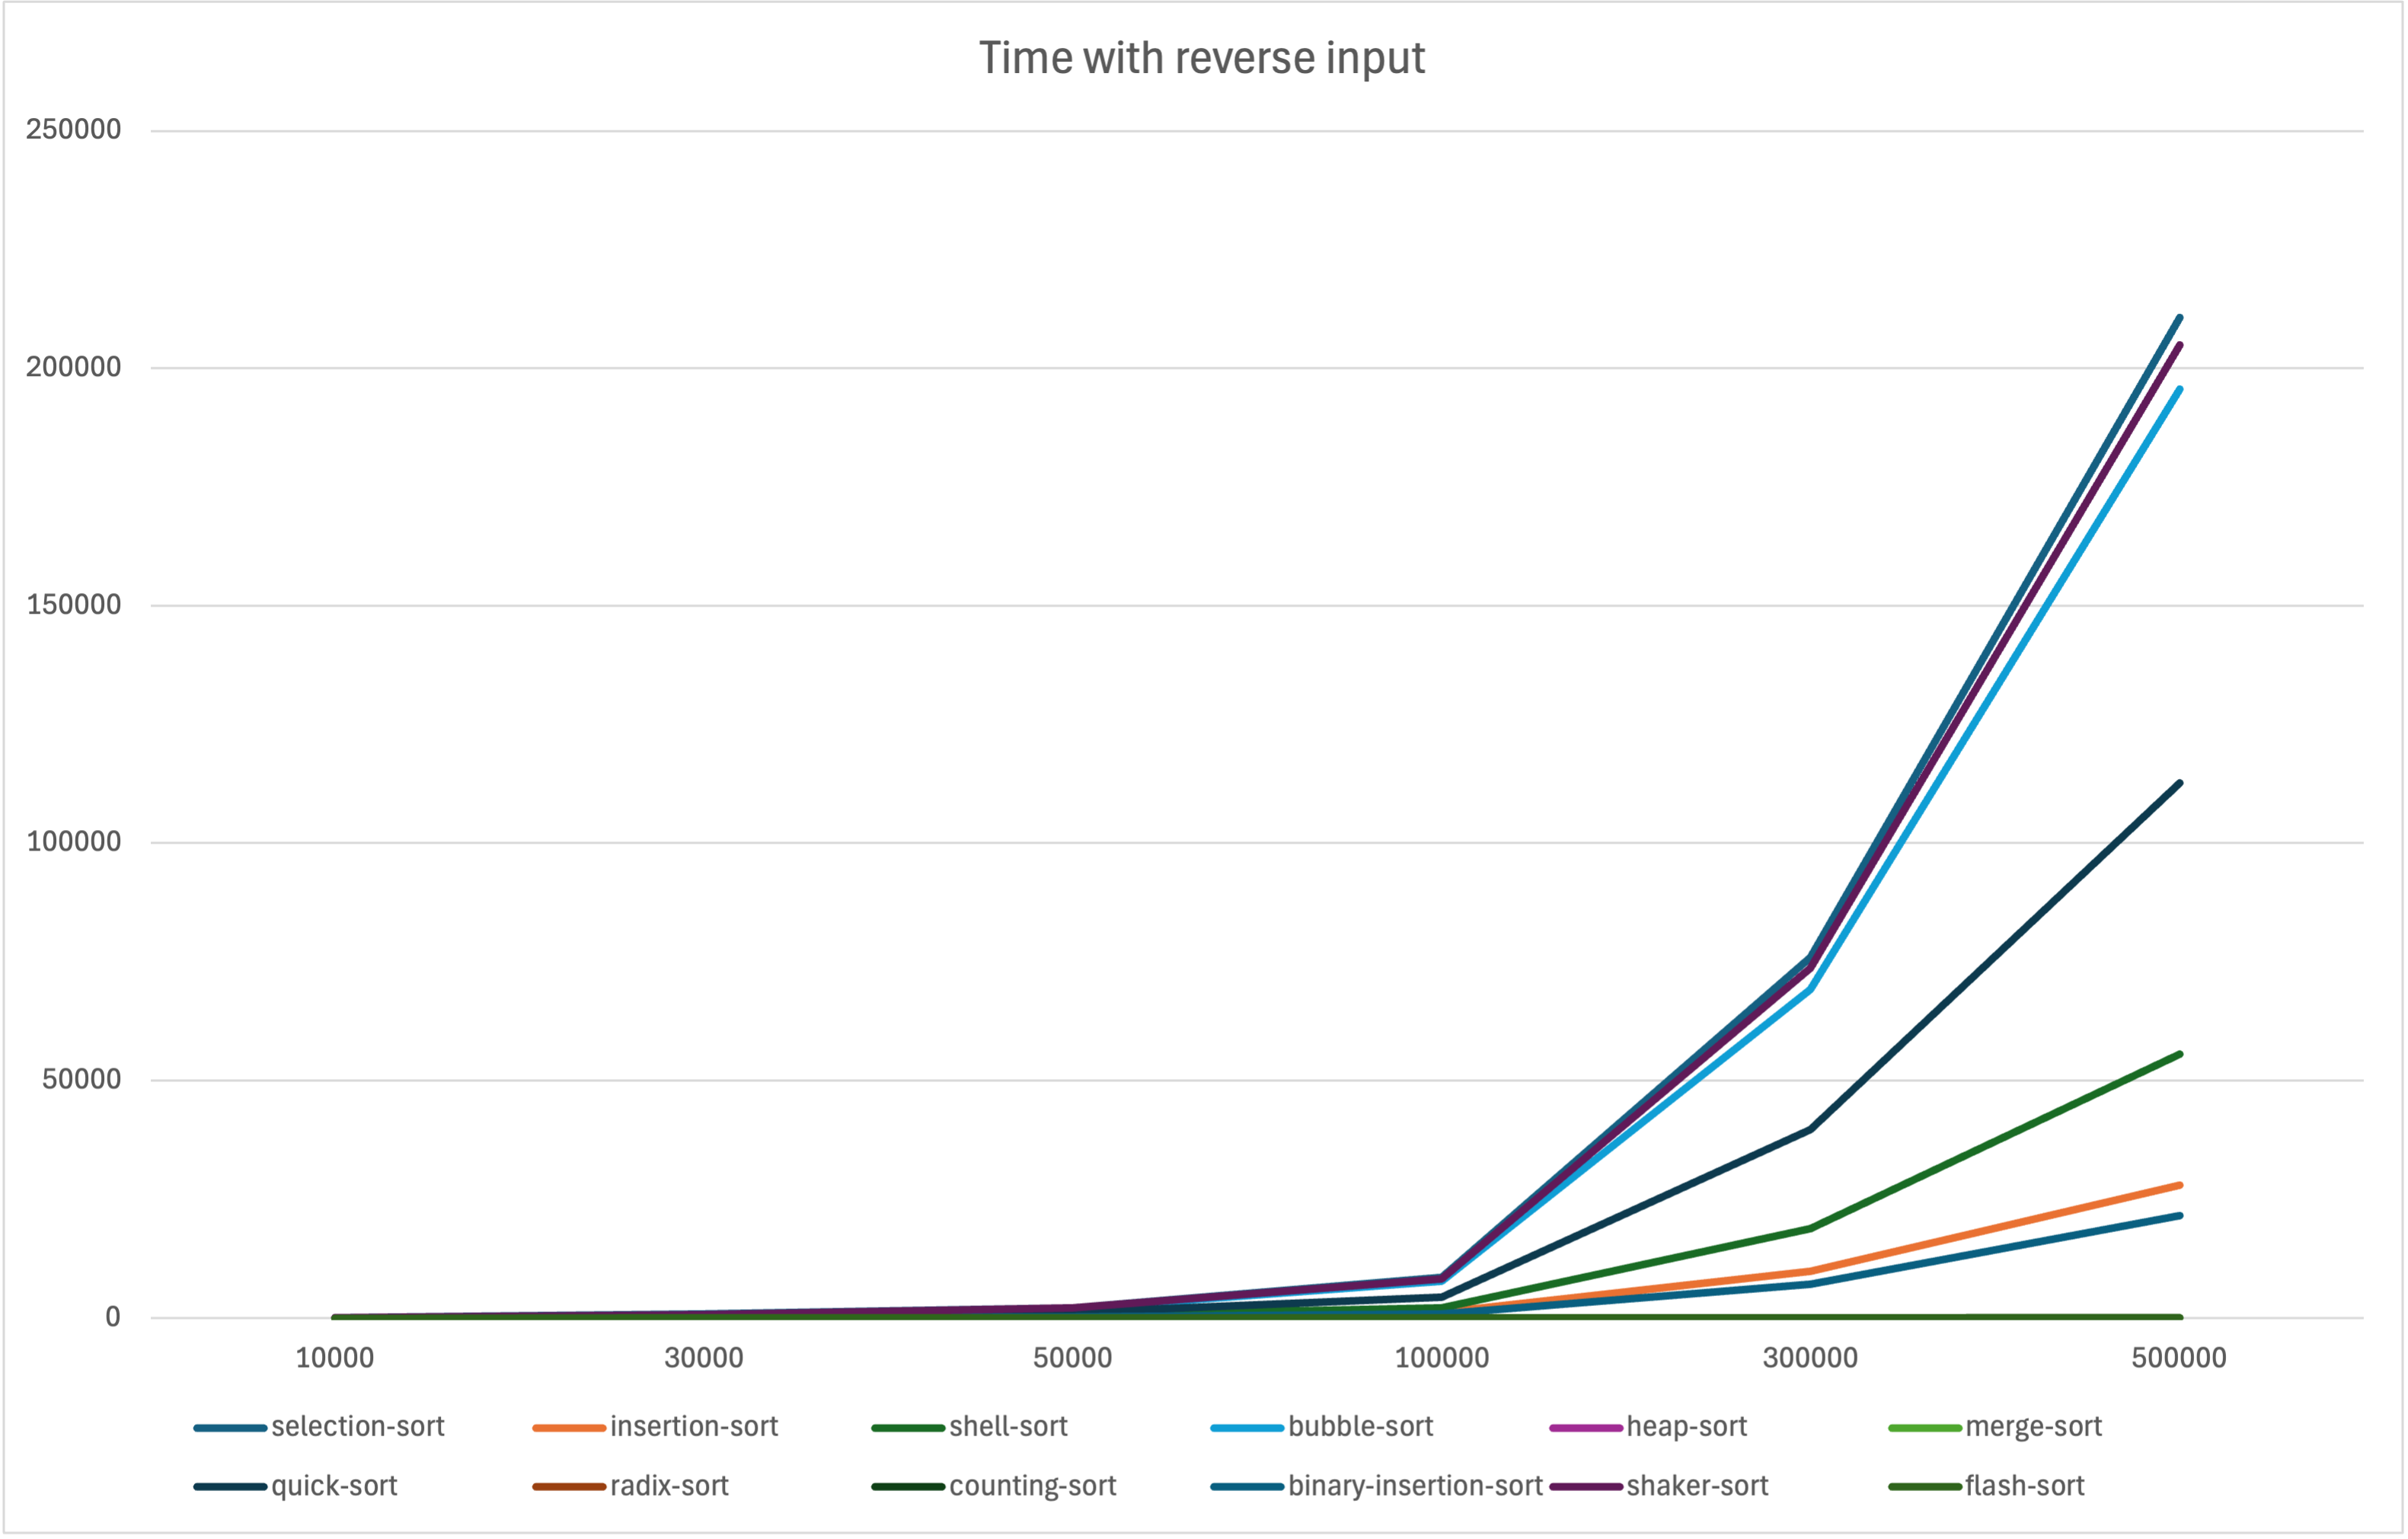
\includegraphics[scale=.65]{Figures/Visualization/Reverse_time.png}
    \caption{Execution time for Reverse data}
    \label{fig:enter-label}
\end{figure}

\subsubsection{Comparison}

\textbf{Comments on the number of comparisons of sorting algorithms with reverse data}
\begin{enumerate}
    \item \textbf{Fewest Comparisons:} \\
- \textit{Counting Sort} and \textit{Radix Sort} consistently perform the fewest comparisons, highlighting their efficiency in this metric for reverse sorted inputs as well.

    \item \textbf{Most Comparisons:} \\
- \textit{Selection Sort}, \textit{Insertion Sort}, \textit{Bubble Sort}, and \textit{Quick Sort} show an extremely high number of comparisons, reaching up to the order of \(10^{11}\) for larger input sizes, indicating significant inefficiency in terms of comparisons.

    \item \textbf{Consistent Performers:} \\
- \textit{Heap Sort}, \textit{Merge Sort}, and \textit{Binary Insertion Sort} maintain a moderate and steadily increasing number of comparisons, showing balanced performance.
\end{enumerate}

\begin{table}[h!]
\centering
\begin{tabular}{|l|r|r|r|r|r|r|}
\hline
\textbf{Algorithm} & \textbf{10000} & \textbf{30000} & \textbf{50000} & \textbf{100000} & \textbf{300000} & \textbf{500000} \\
\hline
Selection Sort & 100020001 & 900060001 & 2500100001 & 10000200001 & 90000600001 & 2.50001E+11 \\ \hline
Insertion Sort & 100009999 & 900029999 & 2500049999 & 10000099999 & 90000299999 & 2.5E+11 \\ \hline
Shell Sort & 136486703 & 1228074234 & 3411144570 & 13643867417 & 1.2279E+11 & 3.41082E+11 \\ \hline
Bubble Sort & 100009999 & 900029999 & 2500049999 & 10000099999 & 90000299999 & 2.5E+11 \\ \hline
Heap Sort & 606771 & 2063324 & 3612724 & 7718943 & 25569379 & 44483348 \\ \hline
Merge Sort & 476441 & 1573465 & 2733945 & 5767897 & 18708313 & 32336409 \\ \hline
Quick Sort & 100019998 & 900059998 & 2500099998 & 10000199998 & 90000599998 & 2.50001E+11 \\ \hline
Radix Sort & 140051 & 510064 & 850064 & 1700064 & 6000077 & 10000077 \\ \hline
Counting Sort & 60003 & 180003 & 300003 & 600003 & 1800003 & 3000003 \\ \hline
Binary Insertion Sort & 50348179 & 451187593 & 1252080140 & 5004460231 & 45014870410 & 1.25026E+11 \\ \hline
Shaker Sort & 100005001 & 900015001 & 2500025001 & 10000050001 & 90000150001 & 2.5E+11 \\ \hline
Flash Sort & 103753 & 311253 & 518753 & 1037503 & 3112503 & 5187503 \\
\hline
\end{tabular}
\label{table:reverse_number_of_comparisons}
\end{table}

\begin{figure}[h]
    \centering
    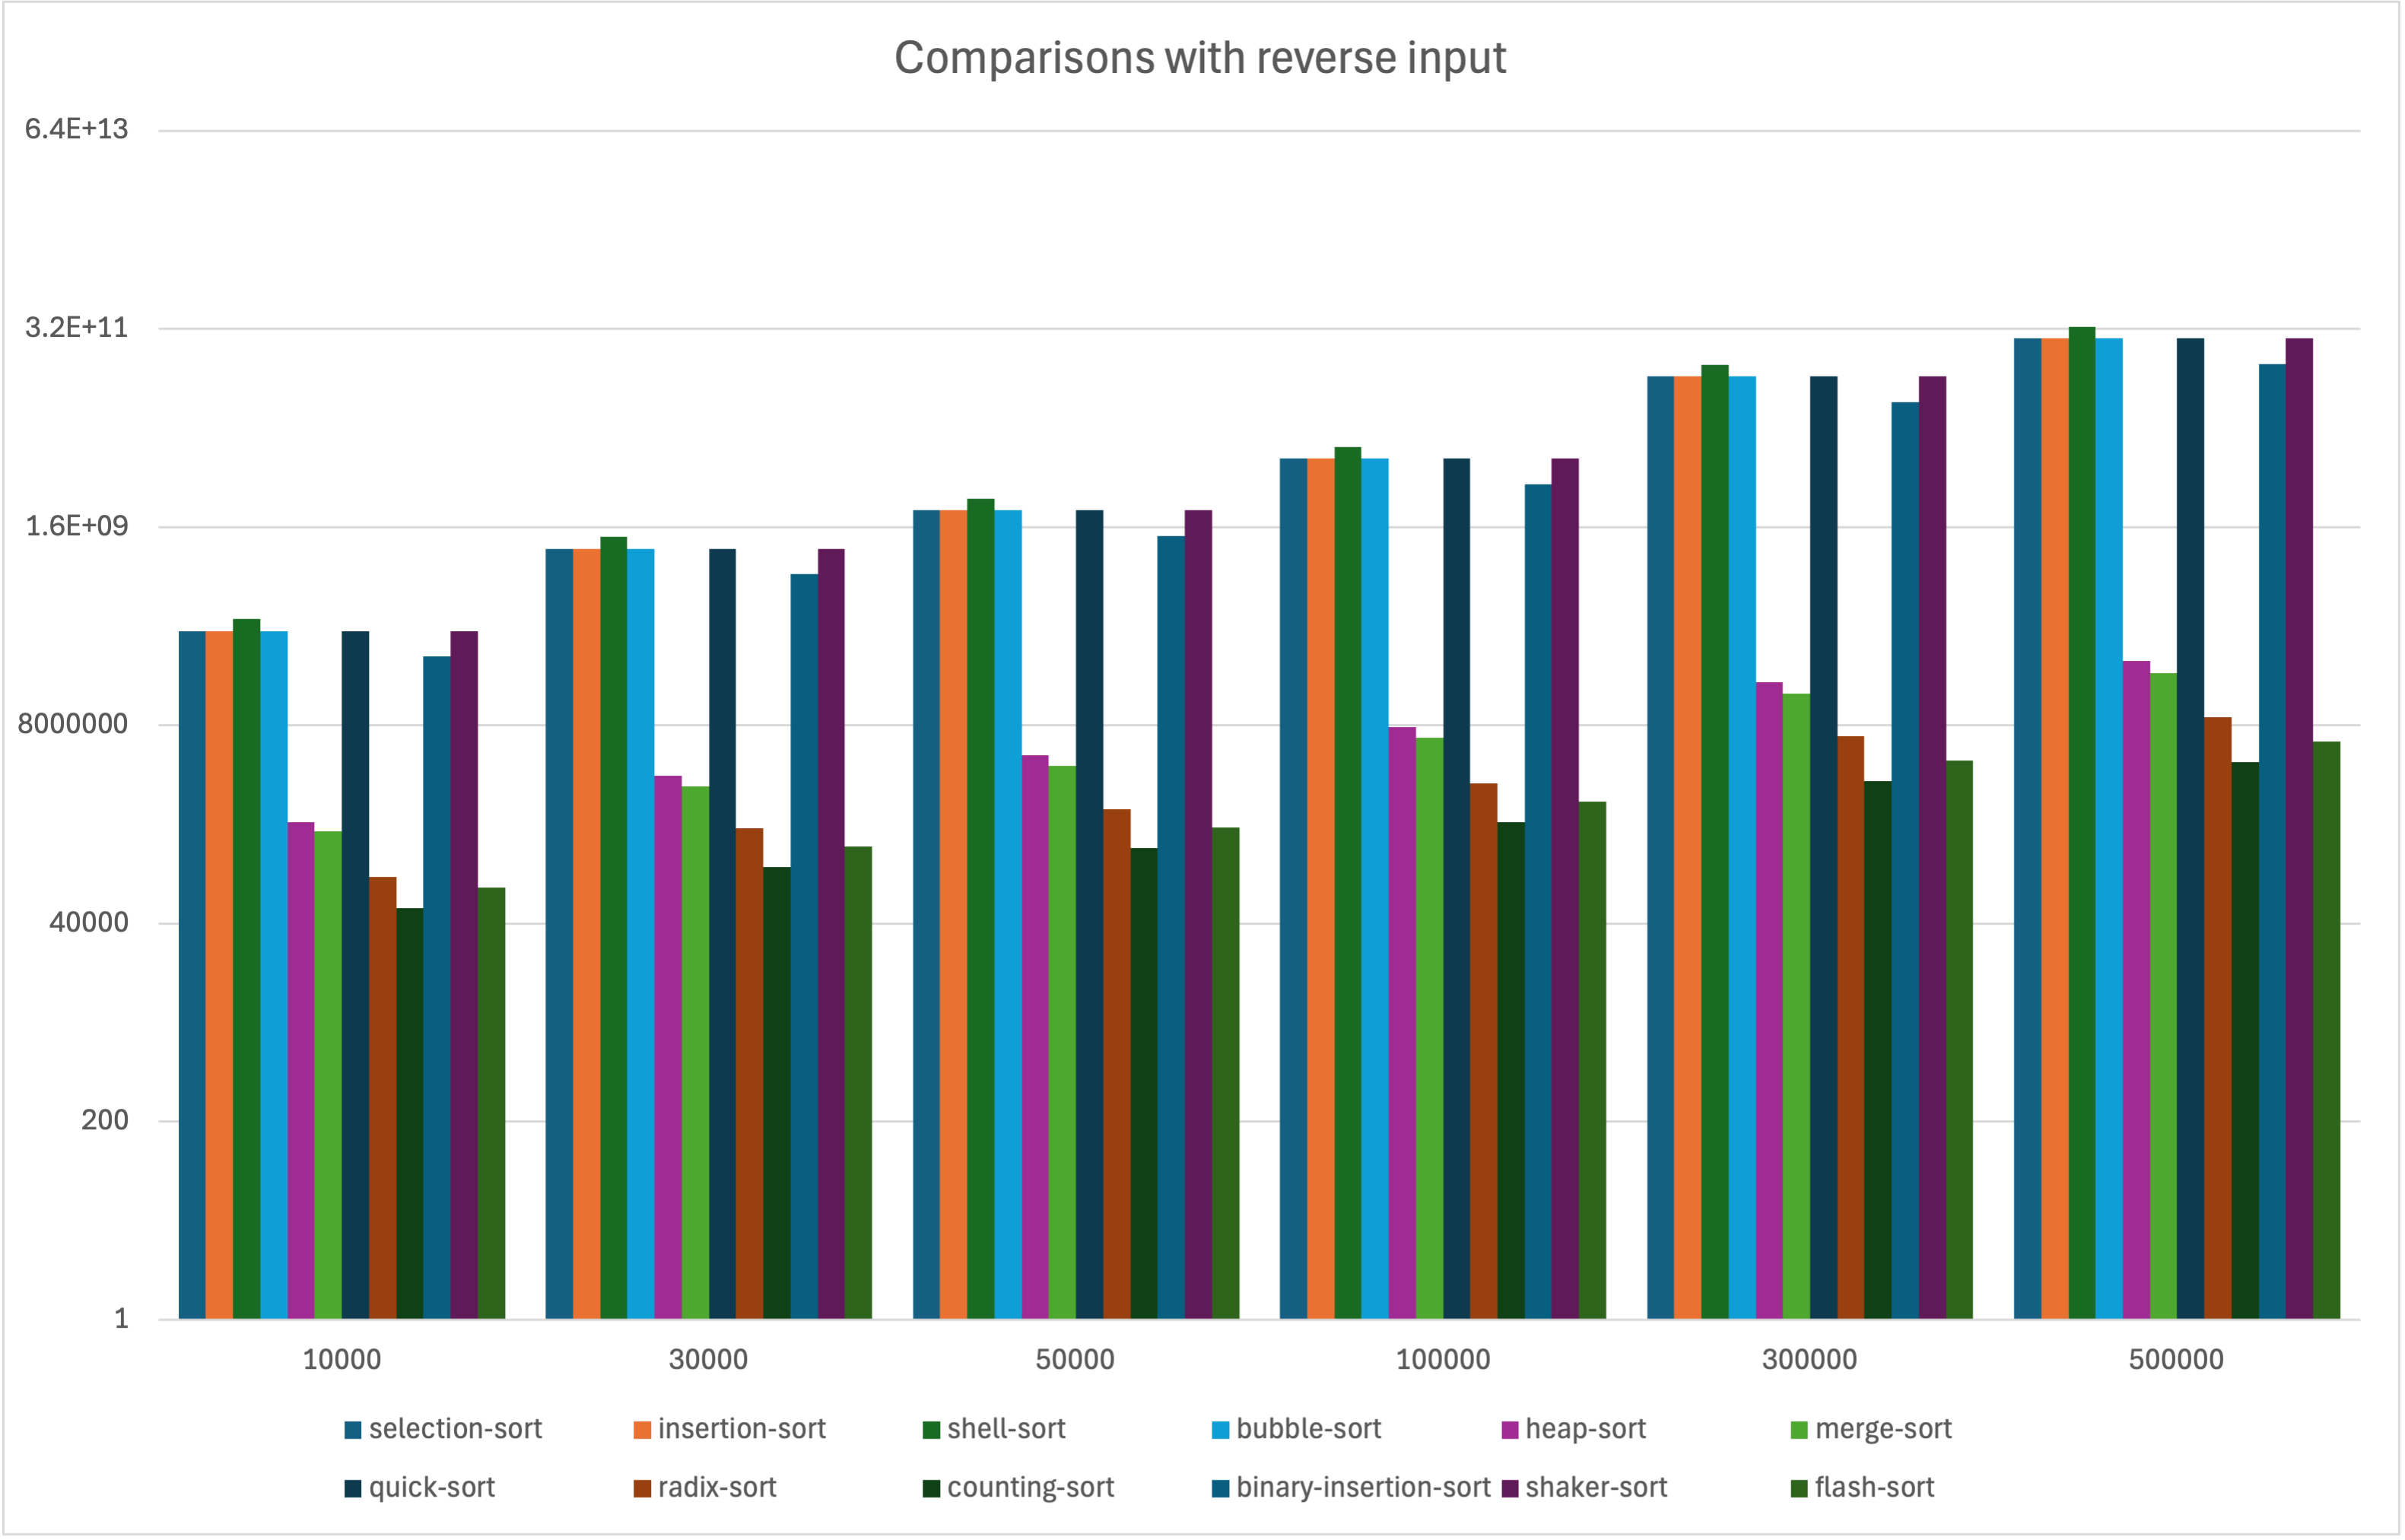
\includegraphics[scale=.65]{Figures/Visualization/Reverse_compare.png}
    \caption{Number of comparisons of the algorithm for Reverse data}
    \label{fig:enter-label}
\end{figure}

\subsubsection{Overall}
\begin{enumerate}
    \item \textbf{Stable Algorithms:} \\
- \textit{Heap Sort}, \textit{Radix Sort}, and \textit{Merge Sort} are stable across both sorted and reverse sorted data in terms of execution time and number of comparisons. These algorithms are generally reliable and efficient.

    \item \textbf{Unstable Algorithms:} \\
- \textit{Quick Sort}, \textit{Selection Sort}, \textit{Bubble Sort}, and \textit{Shaker Sort} are unstable, especially with a significant increase in execution time and number of comparisons as the input size grows. These algorithms tend to be inefficient for larger datasets and in different data orders.

    \item \textbf{Fastest Algorithms Overall:} \\
- \textit{Insertion Sort}, \textit{Counting Sort}, and \textit{Binary Insertion Sort} consistently show the fastest execution times, particularly for smaller input sizes. Their performance is highly efficient for both sorted and reverse sorted inputs.

    \item \textbf{Slowest Algorithms Overall:} \\
- \textit{Selection Sort}, \textit{Bubble Sort}, and \textit{Shaker Sort} are the slowest overall, showing significantly higher execution times and a very high number of comparisons for larger datasets and different data orders.
\end{enumerate}
